\begin{center}
\begin{minipage}[t]{.46\linewidth}\vspace{0pt}\centering
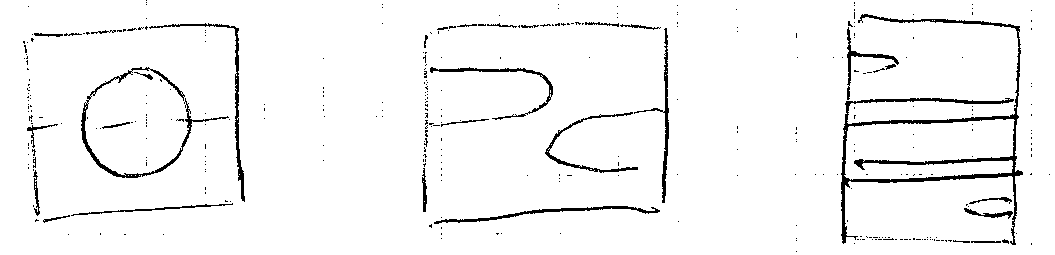
\includegraphics[width=\linewidth]{figures/gelfand-0153-p001408-baker-sequence-original.png}\par\smallskip
{\footnotesize Оригинал рукописного рисунка: \texttt{GELFAND-P001408}}
\end{minipage}\hfill
\begin{minipage}[t]{.50\linewidth}\vspace{0pt}\centering
{\footnotesize Частичное воссоздание видимых штрихов}\par\smallskip
\resizebox{\linewidth}{!}{% Only the clear leftward long arrow is interpreted as a direction.
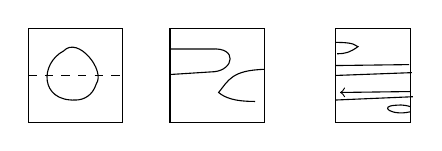
\begin{tikzpicture}[x=.6cm,y=.6cm]
\draw (0,0) rectangle (2,2);\draw[dashed] (0,1)--(2,1);
\draw (1,.48) .. controls (.25,.45) and (.24,1.25) .. (.75,1.52)
 .. controls (1.05,1.84) and (1.64,1.11) .. (1.44,.82)
 .. controls (1.36,.57) and (1.17,.48) .. (1,.48);
\draw (3,0) rectangle (5,2);
\draw (3,1.56)--(3.88,1.56) .. controls (4.44,1.6) and (4.35,1.12) .. (3.94,1.08)--(3,1.02);
\draw (5,1.13) .. controls (4.31,1.11) and (4.24,.9) .. (4.03,.64)
 .. controls (4.16,.53) and (4.36,.45) .. (4.8,.45);
\draw (6.5,0) rectangle (8.1,2);
\draw (6.5,1.7) .. controls (6.93,1.7) and (6.9,1.64) .. (6.98,1.61)
 .. controls (6.81,1.49) and (6.72,1.46) .. (6.54,1.46);
\draw (6.5,1.21)--(8.06,1.23) (6.5,1.0)--(8.12,1.06);
\draw[->] (8.1,.66)--(6.6,.64);\draw (6.5,.48)--(8.14,.55);
\draw (8.08,.23) .. controls (7.7,.14) and (7.4,.35) .. (7.78,.37)
 .. controls (7.93,.39) and (8.07,.35) .. (8.08,.34);
\end{tikzpicture}
}
\end{minipage}
\end{center}
\noindent{\small\textit{Видимые изгибы сохранены. Направление указано лишь у ясно различимой длинной стрелки влево; мелкие конечные штрихи не истолкованы.}}
